%!TEX root = bachelor.tex

\chapter{Architecture}
\label{architecture}

\begin{figure}[ht]
	\centering
	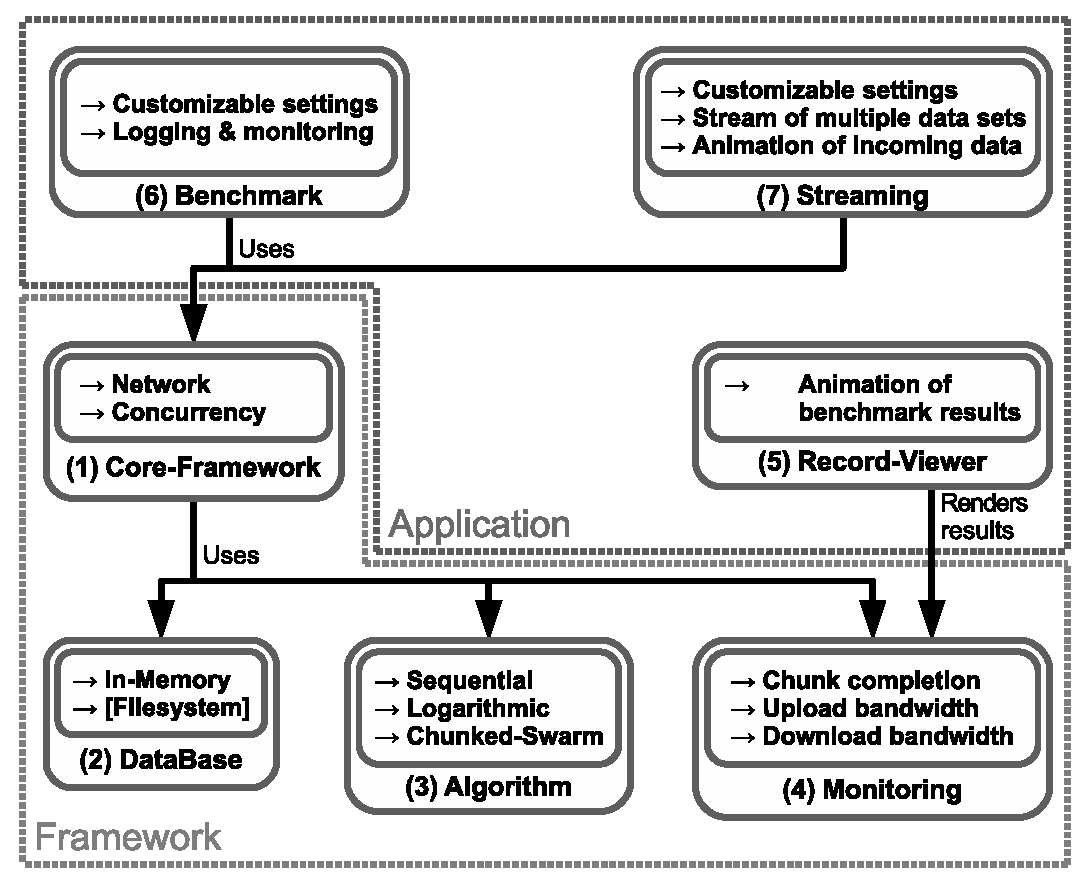
\includegraphics[width=0.8\linewidth]{arch}
	\caption{Software Architecture}
	\label{fig:arch}
\end{figure}

This chapter explains the architecture of the software in detail. From the beginning, one of the main goals were to achieve high modularity, so individual parts can be enhanced or replaced easily. The software is separated into the framework and the application part, which consists of multiple modules. Figure \ref{fig:arch} shows the architecture. 

\vfill
\pagebreak

The application part depends on the Core-Framework and the Monitoring module. It contains three modules which are Benchmark, Streaming and Record-Viewer. The Benchmark module is the most important application part, because it can help to create, monitor and evaluate different scenarios in terms of performance and efficiency. All measurements were done using this module. The Streaming module demonstrates the possibility for an incremental stream of data sets. The Record-Viewer module can render and animate results taken from the Monitoring module, which belongs to the framework part and thus only depends on it.

The Core-Framework, DataBase, Algorithm and Monitoring module are framework modules. While the DataBase, Algorithm and Monitoring module can be replaced or even omitted the Core-Framework module is fundamental. It manages network, concurrency and the communication of the three other modules located in the framework part. The DataBase module represents an interface for a generic data storage, which might be the file system or even completely in-memory. The Algorithm module contains the implementations of the concepts presented in Chapter \ref{theory}. To implement and test new distribution algorithms only this module has to be modified. The Monitoring module records data like current bandwidth usage and chunk completion, which are important data for evaluating the distribution algorithms. This module creates \emph{CSV} files, which can be plotted with tools like \emph{GNUplot}\footnote{http://www.gnuplot.info} and a log file, which contains a chronological stream of events occurred during the recording and can be rendered using the Record-Viewer module.

In the next chapters the framework and application modules are explained in detail. The order is bottom-up, which means the Core-Framework module is explained first in Chapter \ref{module:core} followed by the DataBase and Algorithm in Chapter \ref{module:database} and \ref{module:algorithm} respectively. The Monitoring, Record-Viewer and Benchmark modules are discussed together in Chapter \ref{module:monitoring}. Lastly, the Streaming module is presented in Chapter \ref{module:streaming}.